\documentclass[aspectratio=169]{beamer}
\beamertemplatenavigationsymbolsempty

% The multimedia package is the modern alternative to movie15 and ships with
% Beamer itself.  It exposes the \movie command.  This file exercises the
% most common options so each one can be verified in the generated PPTX.
\usepackage{multimedia}

\title{Beamer with Video (multimedia)}
\author{Author Name}
\date{\today}

\begin{document}

\begin{frame}
    \titlepage
\end{frame}

\begin{frame}{Default --- Click to Play}
    No special options: PowerPoint starts playback when the poster image is
    clicked.
    \begin{center}
        \movie[width=0.7\linewidth,height=0.4\linewidth,poster,showcontrols]
              {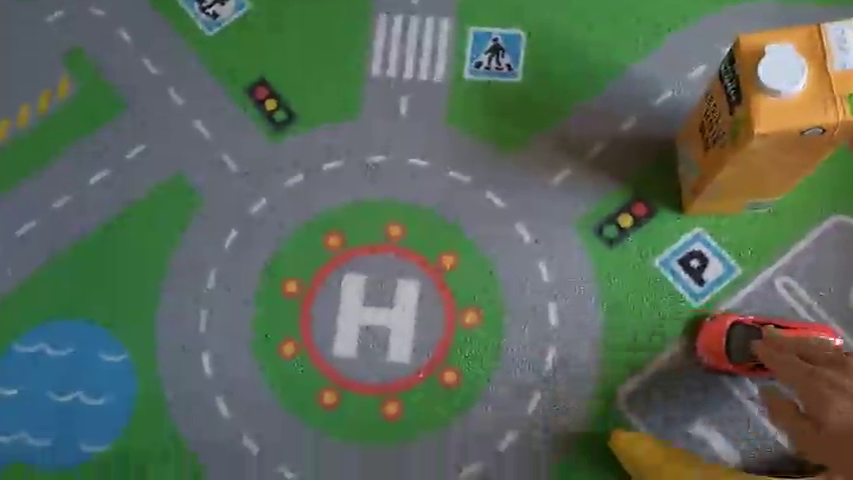
\includegraphics[width=0.7\linewidth,height=0.4\linewidth]{video_snap.png}}
              {video.mp4}
    \end{center}
\end{frame}

\begin{frame}{Autostart}
    The \texttt{autostart} option starts playback automatically when the
    slide becomes visible (equivalent to movie15's \texttt{autoplay}).
    \begin{center}
        \movie[width=0.7\linewidth,height=0.4\linewidth,autostart,showcontrols]
              {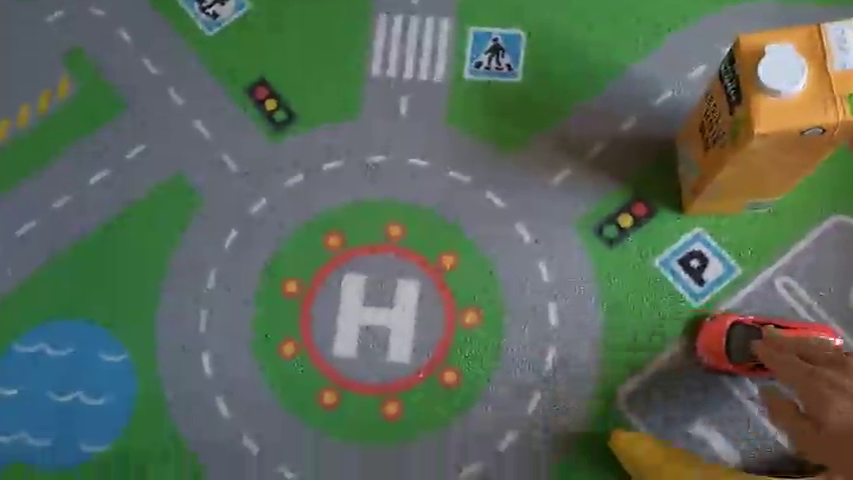
\includegraphics[width=0.7\linewidth]{video_snap.png}}
              {video.mp4}
    \end{center}
\end{frame}

\begin{frame}{Autostart + Loop}
    The \texttt{loop} option causes the video to play continuously.
    \begin{center}
        \movie[width=0.7\linewidth,height=0.4\linewidth,autostart,loop]
              {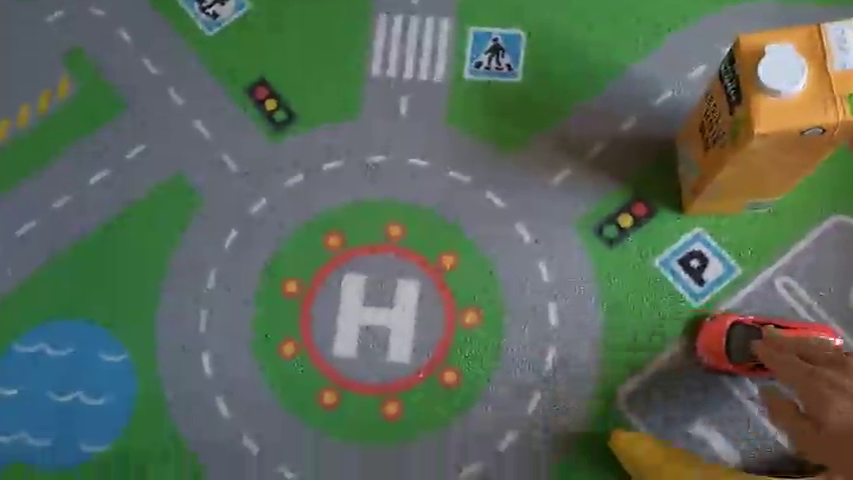
\includegraphics[width=0.7\linewidth]{video_snap.png}}
              {video.mp4}
    \end{center}
\end{frame}

%\begin{frame}{Autostart + Loop}
%    Commented out frame should not affect the result.
%    \begin{center}
%        \movie[width=0.7\linewidth,height=0.4\linewidth,autostart,loop]
%              {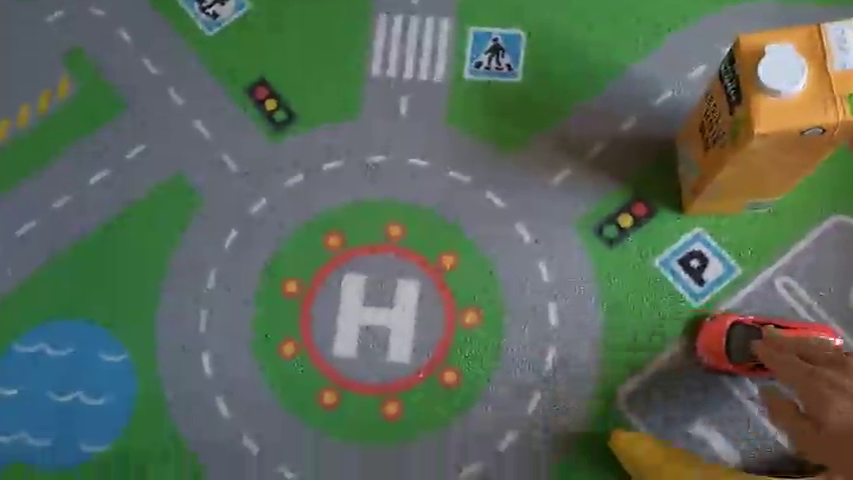
\includegraphics[width=0.7\linewidth]{video_snap.png}}
%              {video2.mp4}
%    \end{center}
%\end{frame}

\begin{frame}{Palindrome (forward then reverse)}
    The \texttt{palindrome} option plays the clip forward then backward.
    PowerPoint's media engine doesn't support reverse playback natively, so
    \texttt{beampptx} maps this to a regular loop.
    \begin{center}
        \movie[width=0.7\linewidth,height=0.4\linewidth,autostart,palindrome]
              {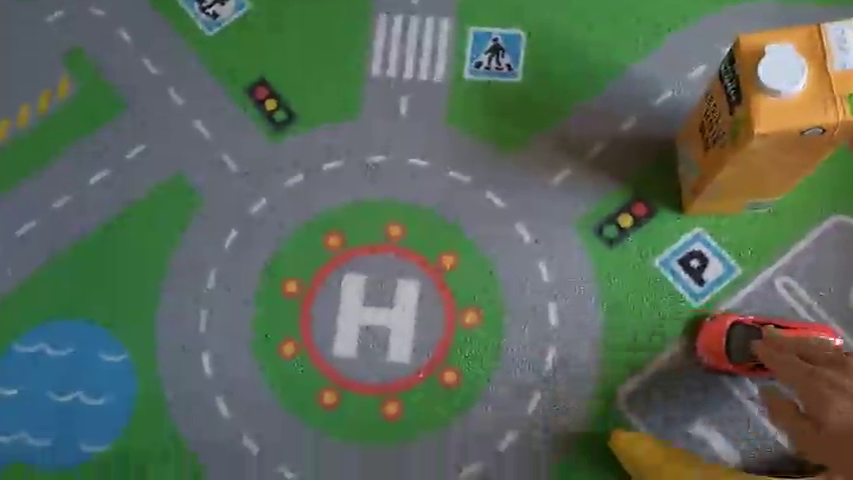
\includegraphics[width=0.7\linewidth]{video_snap.png}}
              {video.mp4}
    \end{center}
\end{frame}

\end{document}